% 6 pages max
\documentclass[twocolumn]{article}
% packages
%\usepackage[utf8]{vietnam}
\usepackage{amsmath, amssymb, amsthm}
\usepackage{color, graphicx, cases}
\usepackage{hyperref}
\hypersetup{
	colorlinks=true,
	linkcolor=blue,
	filecolor=blue,      
	urlcolor=blue,
}
\usepackage{array, multirow, booktabs}
\usepackage{caption, subcaption}
\usepackage{ragged2e} % using justifying
\numberwithin{equation}{section}
\everymath{\displaystyle}
\usepackage{titling}
\usepackage{abstract}

\topmargin=-10mm \headsep=5mm \evensidemargin=-12mm
\oddsidemargin=-6mm \textwidth=170mm \textheight=242mm
\columnsep=6mm

%\usepackage[a4paper,left=35mm,top=31mm,right=20mm,bottom=30mm]{geometry}
%\renewcommand{\baselinestretch}{1.5}

% new definitions
\newtheorem{dl}{Theorem}[section]
\newtheorem{md}{Proposition}[section]
\newtheorem{hq}{Corollary}[section]
\newtheorem{cy}{Remark}[section]

\theoremstyle{definition}
\newtheorem{dn}{Definition}[section]
\newtheorem{vd}{Example}[section]
\newtheorem{bt}{Problem}[section]
\newtheorem{nx}{Comment}[section]

% reference
\usepackage{cleveref}
\crefname{dl}{\textbf{Theorem}}{}
\crefname{md}{\textbf{Proposition}}{}
\crefname{hq}{\textbf{Corollary}}{}

\crefname{dn}{\textbf{Definition}}{}
\crefname{vd}{\textbf{Example}}{}
\crefname{cy}{\textbf{Remark}}{}
\crefname{bt}{\textbf{Problems}}{}
\crefname{nx}{\textbf{Comment}}{} 
\title{\bf Numerical simulation of heat transfer problem by Freefem++ software}
\author{Ta Thi Thanh Mai\thanks{email: tathithanhmai@gmail.com}\and Ho Duc Nhan\thanks{email: hdnhan28@gmail.com}\and Tran Minh Tam\thanks{email: tam.tranminh22@gmail.com}}
%\thanksmarkseries{arabic}
\date{\footnotesize\textit{School of Applied Mathematics and Informatics, Hanoi University of Science and Technology, No.1 Dai Co Viet street, Hai Ba Trung District, Hanoi, Vietnam}}
\justifying
% ---------------------------------------------
\begin{document}
\twocolumn[
	\maketitle
	\begin{@twocolumnfalse}
		\rule{\textwidth}{.1pt}
		\begin{abstract}
			content...
		\end{abstract}
		\vspace{1ex}
		\noindent \textit{Keywords: Inverse source problems, least squares method, Tikhonov regularization, conjugate gradient method.}
		\rule{\textwidth}{.1pt}
		\vspace{2mm}
	\end{@twocolumnfalse}
]
\saythanks

% --------------------------------------------------------------------
\section{Introduction}
% --------------------------------------------------------------------
\quad Let $\Omega \subset \mathbb{R}^d,\, d\in \mathbb{N^+}$ be a bounded domain with a boundary $\Gamma$ and endow the cylinder $Q=\Omega\times (0,\, T]$ and lateral surface area $S=\Gamma \times (0,\, T]$ where $T>0$. 

Consider the heat equation:
\begin{align}\label{1.1}
	\frac{\partial u(x, t)}{\partial t}+\mathcal{L}u(x, t)=F(x, t), \quad(x, t)\in Q,
\end{align}
with the Dirichlet boundary and initial conditions, respectively
\begin{align}
	u(x, t)&=u_D(x, t),\quad(x, t)\in S, \label{1.2}\\
	u(x, 0)&=u_0(x),\quad\quad\, x\in \Omega,\label{1.3}
\end{align}
where
\begin{align*}
	&\mathcal{L}u = -\sum_{i, j=1}^{d}\frac{\partial}{\partial x_i}\left(a_{ji}\frac{\partial u}{\partial x_j}\right)+a_0u,\\
	&a_{ji}\in L^{\infty}(Q),\, a_{ij}=a_{ji},\; \forall i, j\in \{1, 2, ..., d\},\\
	&\lambda_1\left\|\xi\right\|^2\leq \sum_{i, j=1}^{d}a_{ij}\xi_i\xi_j\leq \lambda_2\left\|\xi\right\|^2,\; \forall \xi\in\mathbb{R}^d,\\
	&a_0\in L^{\infty}(Q),\; 0\leq a_0(x, t)\leq \mu_1,\; (x, t)\in Q,\\ 
	&u_0\in L^2(\Omega),\;u_D\in L^2(S),
\end{align*}
with $\lambda_1$ and $\lambda_2$ are positive constants and $\mu_1\geq 0$.
\\
The problem is that to determine $u$ when all data $a_{ji},\,a_0,\,u_0,\,u_D$ and $F$ in \eqref{1.1} - \eqref{1.2} - \eqref{1.3} are given called \textbf{\textit{direct problem}}. 
%But in practice, we miss one of the data above such as  the right hand side $F$ of \eqref{1.1} known for heat source. The problem identifying $F$ when some additional observations on the solution $u$ available called \textbf{\textit{inverse problem}}. We suppose that the heat source following the form $F(x, t)=f(x, t)q(x, t)+g(x, t)$, where $q(x, t),\, g(x, t)$ are given. Find $f(x, t)$ if $\omega(x, t)=u(x, t)$ is given on $Q$. 
% --------------------------------------------------------------------
\section{Numerical method} 
% --------------------------------------------------------------------
\subsection{Variational problem}
% --------------------------------------------------------------------
\quad Multiplying \eqref{1.1} by an efficient smooth test function $v$, integrating over $\Omega$ and then applying Green's formula, see \cite{}, leads to the problem: Find $u(.,t)\in H^1(\Omega)$ such that
\begin{align}\label{2.1}
	\left\langle \frac{\partial u}{\partial t}, v \right\rangle+a\left(u, v\right)=\left\langle F, v \right\rangle,\; \forall v\in H^1(\Omega),
\end{align} 
\begin{align}\label{2.2}
	u(x, 0)=u_0(x), \; x\in \Omega,
\end{align}
where 
$$a\left(u, v\right)=\int_{\Omega}\left[\sum_{i, j=1}^{d}a_{ji}\frac{\partial u}{\partial x_i}\frac{\partial v}{\partial x_j}+a_0uv\right]dx,$$
$$\left\langle F, v \right\rangle=\int_{\Omega}F vdx.$$

\subsection{Finite element method}
\quad Now we present a fully discrete finite element approximation for the variational problem \eqref{2.1} as follows:
\begin{itemize}
	\item For \textit{spatial approximation}, let $\mathcal{T}_h$ be a triangulation of $\Omega$ and define a piecewise linear finite element space $V_h \subset H^1(\Omega)$ by
	$$V_h=\left\{v_h:v_h\in C(\overline{\Omega}), v_h|_K\in P_1(K), \forall K\in \mathcal{T}_h\right\},$$
	where $P_1(K)$ is a continuous piecewise linear polynomial on the element $K$.
	\item For \textit{temporal discretization}, discrete $[0, T]$ uniformly into $M$ steps, $t_n=n\Delta t,\, n=0, 1, \dots, M$ with the time step size $\Delta t = T/M$. We define a function $u(x, t_n)=u^n(x)$.
\end{itemize}

Find $u^n_h\in V_h$ for $n=1, 2, \dots, M$ with $\theta \in [0, 1]$ such that
\begin{align}\label{2.3}
	&\langle d_tu^n_h, v_h \rangle+a\left(\theta u^n_h+(1-\theta)u^{n-1}_h, v_h\right)\notag\\
	&\qquad\quad=\left\langle \theta F^n+(1-\theta)F^{n-1}, v_h \right\rangle, \; \forall v_h\in V_h,
\end{align}
and the initial condition 
\begin{align}\label{2.4}
	u^0_h=u_0,
\end{align}
where $d_tu^n_h=\frac{u^n_h-u^{n-1}_h}{\Delta t}, \; n=1, 2, ..., M$.

The discrete variational problem \eqref{2.3} -\eqref{2.4} admits a unique solution $u^n_h\in V_h$, see \cite{}. Let $u_h(x, t)$ be the linear interpolation of $u_h^n$ with respect to $t$. Therefore, for $x\in \Omega,\, t\in [t_{n-1}, t_n]$, we have
\begin{align*}
	u_h(x, t)=\frac{t-t_{n-1}}{\Delta t}u_h^{n-1}+\frac{t_n-t}{\Delta t}u_h^{n}.
\end{align*}
\begin{dl}\label{dl2.1}
	Let $u(x, t)$ be the solution of variational problem \eqref{2.1} - \eqref{2.2} and $u^n_h\in V_h$ for $n=1, 2, \dots, M$ be the solution for \eqref{2.3} - \eqref{2.4}. Then there holds the error estimate, see \cite{}
	\begin{align}\label{2.5}
		\left\|u_h-u\right\|_{L^2(Q)}=
		\begin{cases}
			O\left(h^2+\Delta t\right), &\theta=\{0, 1\},\\
			O\left(h^2+\Delta t^2\right), &\theta=\{0.5\},
		\end{cases}		
	\end{align}
	where $h$ is the mesh size.
\end{dl}



% --------------------------------------------------------------------
\section{Tests and discussion}
% --------------------------------------------------------------------
\subsection{Error evaluation with exact solution}
We study a numerical experiment with the exact solution of heat equation and evaluate the error convergence. Consider a square $[0,1]\times[0,1]$. Find $u(x,y,t)$ satisfy
\begin{equation}
\dfrac{\partial u}{\partial t} - \left(\dfrac{\partial^2 u}{\partial x^2} + \dfrac{\partial^2u}{\partial y^2}\right) = (1+2t)\sin(\pi x) \sin(\pi y)
\end{equation}
with the initial and boundary conditions
$$
u(x,y,0) = 0 \quad \text{and} \quad u|_\Gamma = 0.
$$
The exact solution is
$$
u = \sin(\pi x) \sin(\pi y) t,
$$
\begin{figure}[h!]
	\centering
	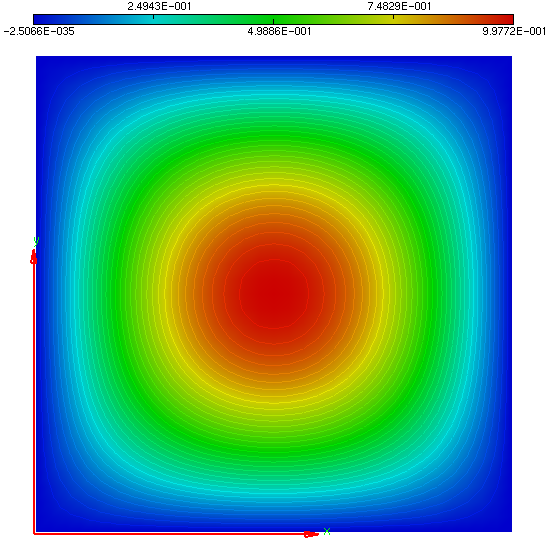
\includegraphics[width=\linewidth]{direct}
\end{figure}
Different cases of mesh size and time step length were studied to show the dependent of error on the mesh smoothness. We also use two different schemes
\begin{itemize}
	\item Backward Euler scheme
	\begin{figure}[h!]
		\centering
		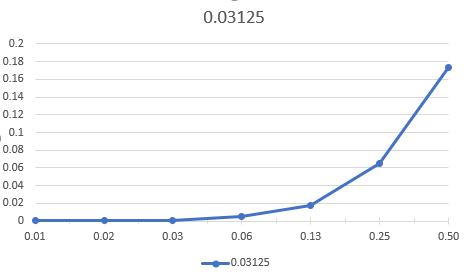
\includegraphics[width=\linewidth]{graph}
	\end{figure}
	\item Crank-Nicolson scheme
\end{itemize}
The approximate solution at final time is illustrated below.
\subsection{A problem of thermal engineering}
In the aspect of thermal engineering, the simulations of heat transfer attend in several applications. In [...] the author mentioned a realistic heat problem which can be solve by simulating the heat transfer process.\\
Assuming there are two types of material with different thermal conductivity and price. We would like to build a thermal resistance wall from composite plate of the two materials that provide optimal thermal resistance properties and satisfies economical conditions. Let $V$ is the total volume of the plate, $V_e$ and $V_c$ are the volume of expensive and cheap material respectively, then the ratio
$$
\mu = \dfrac{V_e}{V} = \dfrac{V_e}{V_c + V_e}
$$
is fixed. Consider a rectangular room $\Omega_r$ has the size $L_x \times L_y$. At the center of the left wall located a radiator that keep the local temperature at $T_r$, denote as $\Gamma_r$, otherwise as $\Gamma_\alpha$. The thermal flux through the walls is expected to be zero, equivalent to the Neumann boundary condition
$$
\dfrac{\partial u}{\partial n} = 0 \quad \text{on} \quad \Gamma_\alpha.
$$
The right corner of the room is where we place our composite thermal resistance plate. Let $\l_x$ is the width of the plate. The right wall is consider the heat source and gain the Dirichlet boundary condition
$$
u = u_{ext} \quad \text{on} \quad \Gamma_{ext}.
$$
Finally, let $\kappa_a, \kappa_c$ and $\kappa_e$ is correspondingly the thermal conductivity coefficient of air, our cheap and expensive material. Based on our goal of minimizing the temperature inside the room, the cost function can be formulated as follow
$$
J = \dfrac{1}{|\Omega_a|}\int_{0}^{T} \int_{\Omega_a} u dx 
$$
This problem belong to the set of shape optimization problems or more generally is an inverse heat problem. These kinds of problems take part in large amount of engineering applications. An approach is to solve as much acceptable input cases as possible then determine which one is the optimal solution. This way requires numerous computations.


\subsection{Numerical experiment of optimal control problem}
\subsubsection{Optimal control problem}
\quad In engineering, sometimes we want to know how much heat source provided to receive heat $u(x, t)$ in a physical domain $\Omega$ in a time period $[0, T]$ equals or approximates with $\hat{u}(x, t),\, (x, t)\in Q.$ We suppose that heat source following the form $F(x, t)=f(x, t)+q(x, t)$. This leads to optimize the functional
\begin{align}\label{J}
	J(q)=\frac{1}{2}\left\|u-\hat{u}\right\|_{L^2(Q)}^2+\frac{\gamma}{2}\left\|q\right\|_{L^2(Q)}^2,
\end{align}
where $q$ being the control variable and $\gamma>0$ being a regularization parameter.

To solve this problem, we use FreeFem++ software which provides an efficient tool called IPOPT. It is designed to perform optimal control problems, for more details see at \cite{}. To use this optimizer, we need to include the \textit{ff-Ipopt} dynamic library. The parameters including the objective function $J(f)$ and its gradient $\nabla J(f)$ following, see \cite{}
\begin{align}\label{gradJ}
	\nabla J(q)=z(x, t)+\gamma q(x, t),
	\end{align}
	where $z(x, t)$ is the solution of the adjoint problem
	\begin{align}\label{adjoint} 
	\begin{cases}
		-\frac{\partial z(x, t)}{\partial t}+\mathcal{L}z(x, t)=u-\hat{u}, & (x, t)\in Q,\\
		z(x, t)=0, & (x, t)\in S\\
		z(x, T)=0, & x\in \Omega.
	\end{cases}
\end{align}

\subsubsection{Numerical results}
\quad In this section, we experiment an example as in \cite{}. We use finite element method with $\theta=0.5$ known for Crank-Nicolson method to solve the direct problem \eqref{1.1} and adjoint problem \eqref{adjoint}. Consider $\Omega=(0, 1)^2$ and $T=0.1$ and homogeneous Dirichlet boundary condition. The right hand side $f$, the desired state $\hat{u}$ and the initial condition $u_0$ such that
\begin{align*}
	&f(x, t)=-\pi^4w_b(x, T),\\
	&\hat{u}(x, t)=\frac{b^2-5}{2+b}\pi^2 w_b(x, t)+2\pi^2w_b(x, T),\\
	&u_0(x)=\frac{-1}{2+b}\pi^2w_b(x, 0),
\end{align*}
where $w_b(x, t)=e^{b\pi^2 t}\sin(\pi x_1)\sin(\pi x_2), \; b\in \mathbb{R}$.

We chose the regularization parameter $\gamma=\pi^{-4}$ and the optimal solution triple $(\bar{q}, \bar{u}, \bar{z})$ of the optimal control problem \eqref{J} is given by
\begin{align*}
	&\bar{q}(x, t)=-\pi^4\left[w_b(x, t)-w_b(x, T)\right],\\
	&\bar{u}(x, t)=\frac{-1}{2+b}\pi^2w_b(x, t),\\
	&\bar{z}(x, t)=w_b(x, t)-w_b(x, T).
\end{align*}

First, we consider the behavior of the error for a sequence of discretization with decreasing size of the time steps and a fixed spatial triangulation with $N=1089$ nodes. Second, we examine the behavior of the error under refinement of the spatial triangulation for $M=1024$ time steps. We choose the free parameter $b$ to be $-\sqrt{5}$.

\begin{figure}[h!]
	\centering
	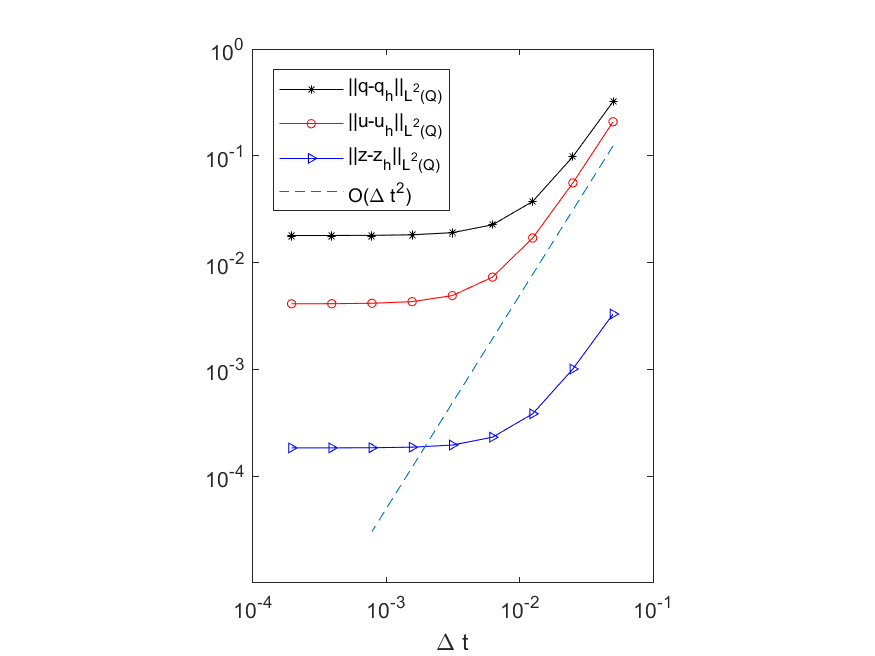
\includegraphics[width=\linewidth]{figures/err_t}
	\caption{Refinement of the time steps for $N =1089$ spatial nodes}
\end{figure}

\begin{figure}[h!]
	\centering
	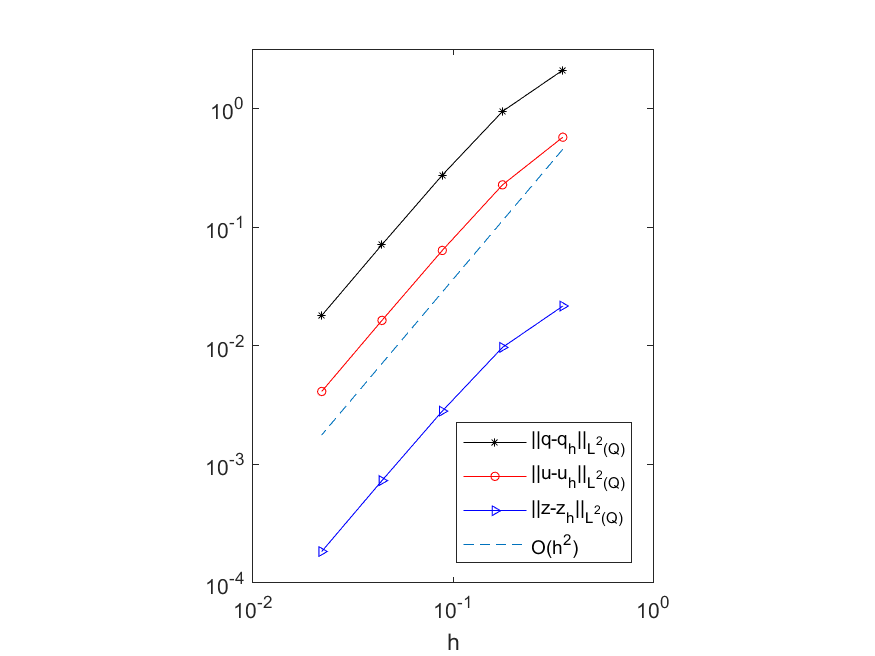
\includegraphics[width=\linewidth]{figures/err_x}
	\caption{Refinement of the spatial triangulation for $M = 1024$ time steps}
\end{figure}



% --------------------------------------------------------------------
\section{Conclusion}
% --------------------------------------------------------------------


% --------------------------------------------------------------------
% biblio
% --------------------------------------------------------------------
\bibliographystyle{plain}
\bibliography{references}{}
\vfill

\end{document}
